\chapter{METHODOLOGY}
\label{ch:methodology}

The proposed self-distillation method training process is shown in Figure~\ref{fig:methodology}.
The first step in training process is to train the image-text representation head by freezing both image and text encoder model as shown in Figure~\ref{fig:methodology} a).
The second step is self-distillation with combined text and image representation output from the image-text representation head as shown in Figure~\ref{fig:methodology} b).
We experiment with multiple image and text encoder models.
We compare our self-distillation method with the self-distillation from the teacher model directly without any text encoder model.
The detail in each part of the expeirment is provided in this section.

\begin{figure}[h]
    \caption{Training methodology}
    \label{fig:methodology}
    \begin{center}
        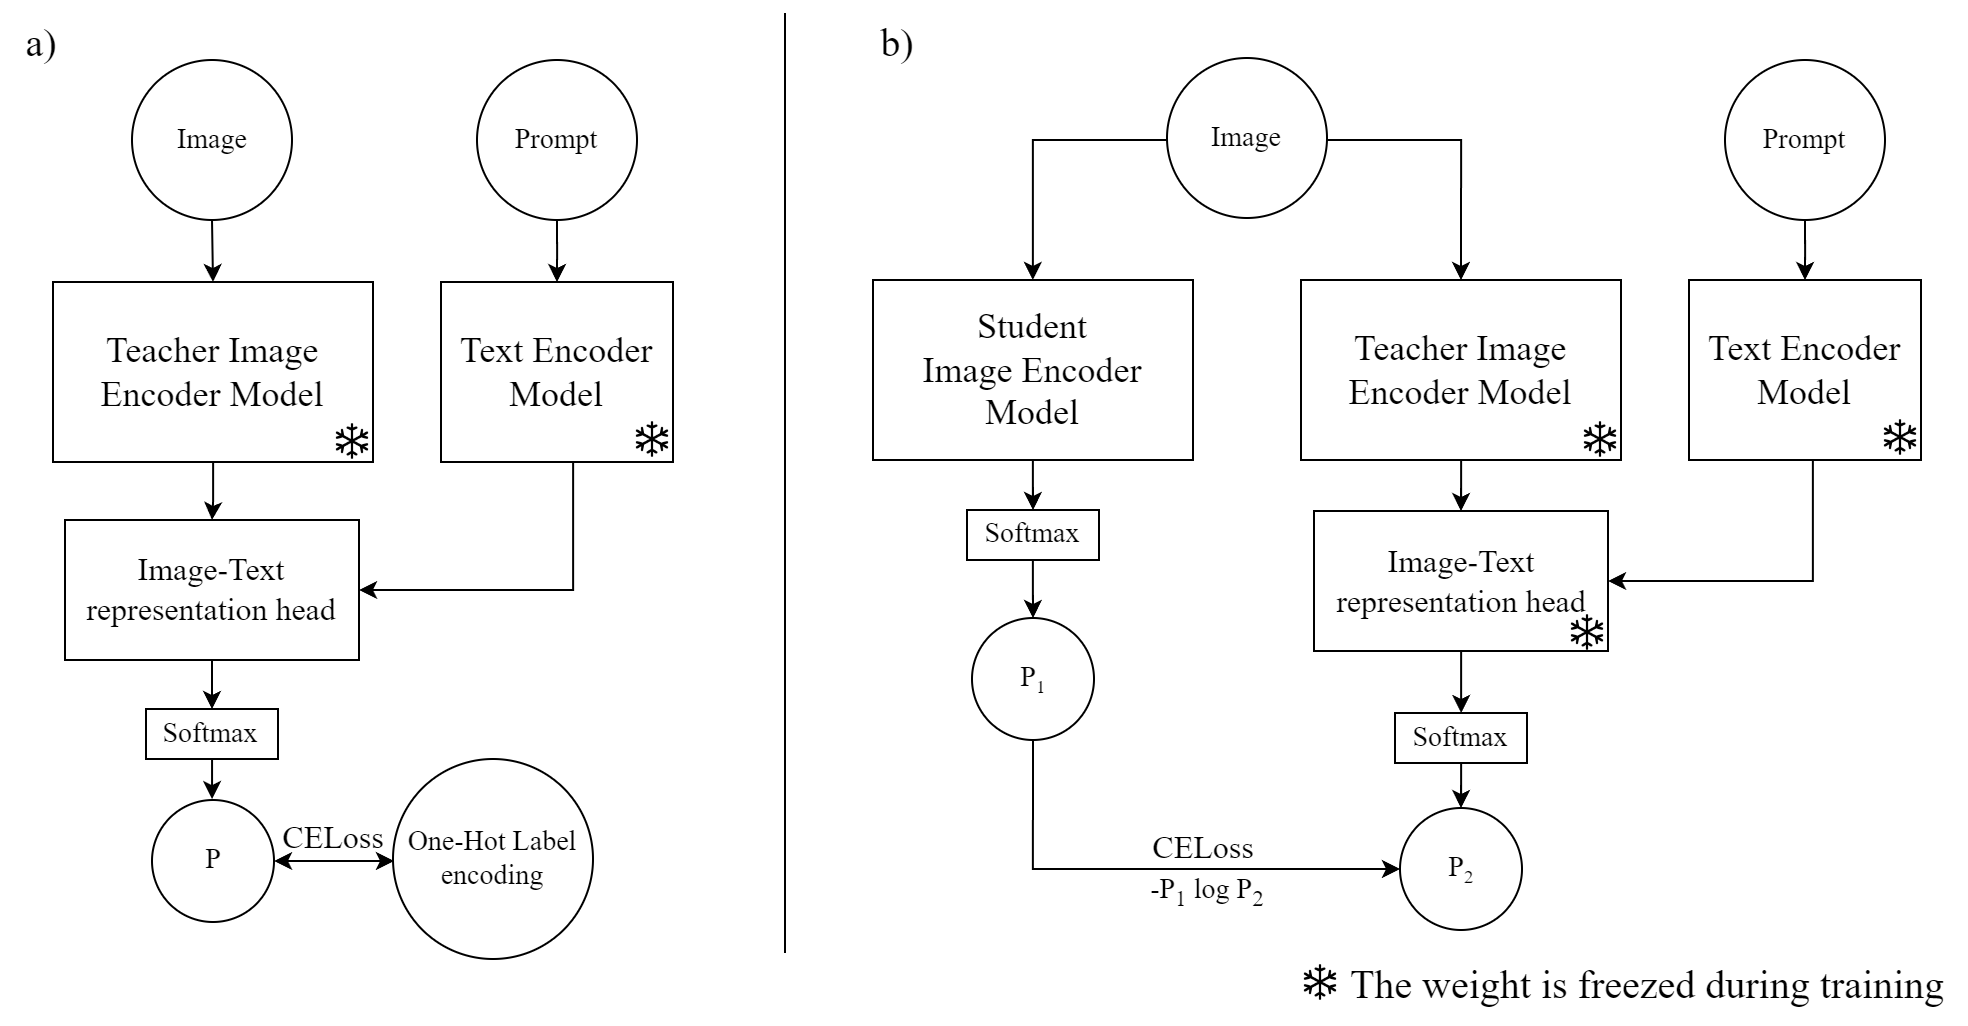
\includegraphics[width=1\textwidth]{Images/Methodology.png}
    \end{center}
    \small a) Training image-text representation head using cross entropy loss b) Self-distillation training by freezing all teacher model
\end{figure}

\begin{figure}[h]
    \caption{Image-Text Cross Attention Classification head}
    \label{fig:cross_attention}
    \centering
    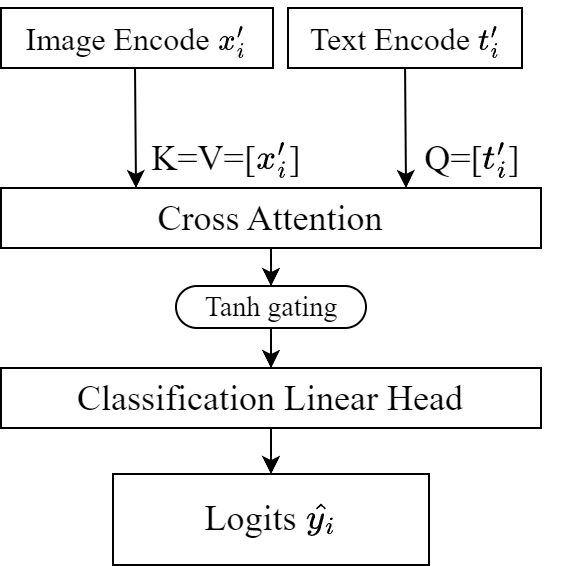
\includegraphics[width=0.5\textwidth]{Images/CrossAttention.png}
\end{figure}

\section{Dataset}
test2

\section{Model Achitecture}
\subsection{Image-text representation head}
By using two encoder model for vision and language individually, the image-text representation have be created to get a single image representation for every single images.
In this experiment, the cross-attention \shortcite{alayrac2022flamingo} architecture with the linear classification head is used to create image-text representation as illustrated in Figure \ref{fig:cross_attention}.

\subsection{Teacher student}
For the teacher model, we will use two stream encoder based model same as CLIP model \shortcite{dosovitskiy2021an}.
In this experiment, the teacher vision encoder model will be ResNet \shortcite{he2016deep} and ViT \shortcite{dosovitskiy2021an} version.
For the student model we used the same architecture as teacher vision encoder model, which are ResNet and ViT.
\textcolor{red}{todo: Add table describes both image and text encoders.}

\section{Training Objectives}
In the first step, we trained the image-text representation head with benchmark datasets by using Cross Entropy loss as describe in \ref{fig:overall_method} a). The image and text encoder was freezed during the first step training. For text input, we used "This is the image of [Class]" as a prompt \shortcite{radford2021learning}. After the first image-text representation head were trained, we create a new student model which have the same architecture as a image encoder model with a linear classification head. The student model was randomly initialized parameters. The objective for self-distillation with teacher and student is


\section{Evaluation}
\section{Ablation Study}

